\documentclass[a4paper,10pt,twocolumn]{article}

\usepackage[a4paper,margin=0.78in]{geometry}
\usepackage[utf8]{inputenc}
\usepackage{amssymb}
\usepackage{amsmath}
\usepackage{graphicx}
\usepackage{wrapfig}
\usepackage{hyperref}
\usepackage{float}
\usepackage{xcolor}
\usepackage{listings}
\usepackage{multirow}
\setlength\parindent{0pt}

\title{Entity Linking Project}
\author{\Large{The Julias}\\Jan Deriu | Rolf Jagerman | Alexey Kustov | Dina Zverinski}

\begin{document}
\maketitle

\section{Problem Statement}
Given a set of real search queries, the task is to automatically annotate the queries with Wikipedia entities. This task includes finding the correct segmentation of the queries as well as the correct entities for the spots. The results are evaluated in terms of precision, recall and F1 scores, which can be computed from manual annotations to the given search queries.

To annotate queries we have implemented numerous algorithms. In the following sections we will explain the ideas behind our approaches and their results.

\section{Failed Approaches}
\subsection{Wikipedia Categories}
The idea was to determine the similarity of two entities by looking at the overlap of the categories they belonged to. To further increase the quality we took into account the links: should one entity link to the other one, we increase the similarity score and should there be a link back the score is increased even more.
We ran into problems with getting the data of the categories. We then decided to use the Wikipedia API to query the categories, which takes a long time, so we decided to filter the crosswikis file by looking only at entries with prior greater than 0.01. However this lead to a very reduced crosswikis file with only 70,000 entities.
This lead to a very low F1 score, since for many annotations the correct entity was not in the filtered crosswikis file.  

\subsection{Bruteforce Similarities}
For this approach, all combinations of possible annotations of all $n$-grams are generated. These annotations are the top 3 entities for every mention starting with the highest prior, taken from the crosswikis file. To find the best combination, a score is computed for each one that is determined by the sum of a similarity score between each two annotations in each combination. Two types of similarity scores have been tested: occurrence counts (i.e. the number of times two entities occur in the same Wikipedia article) and Tagme relatedness. If there is a tie, the best combination is determined by the sum of the prior and length of each annotation.
However, similarity turned out not to be the best indicator for annotations, as many queries are very simple, but may consist of entities that do not have semantic similarity (e.g. "hartford tourism").

\section{Working Approaches}
\subsection{Heuristics}
The heuristics approach uses the naive annotator and attempts to improve on it. Similar to the naive approach, we annotate greedily by spot length, but additionally perform the following steps which helped improve performance:
\begin{itemize}
\item Lowercase all mentions in the crosswikis and queries.
\item Remove special characters (anything not alphanumerical).
\item Remove mentions that start or end with a stopword.
\end{itemize}

On top of these changes, we used a processed version of the crosswikis file created by the "EntityRangers" group. This file has updated names of some of the entities, to make them more similar to the ground truth. For example: "Mozilla Firefox"  $\rightarrow$ "Firefox".

\subsection{Topic Modeling}
The idea of using topic modeling is to exploit the knowledge about topics of the queries and entities. For a potential candidate entity we can compute the distance between it and the query:
\begin{flalign*}
x =&\,\, \parbox[t]{6cm}{A bag-of-word representation of text (an entity's wikipedia page or a query's search results snippets)}\\
\text{topics}(x) =&\,\, \parbox[t]{6cm}{$K$-dimensional probability vector representing the topics of $x$}\\
d(q,e) =&\,\, \text{cosinedistance}(\text{topics}(q), \text{topics}(e))
\end{flalign*}

In order to obtain the topics of all entities and queries we have trained a latent dirichlet allocation (LDA) model on the entire Wikipedia corpus. We used the Vowpal Wabbit implementation \cite{vw}, which uses feature hashing and streaming to reduce the memory requirements. The trained model is used to compute the topic-probability vectors of every entity and query.

Using only the cosine distance between topic vectors of queries and entities is not sufficient to accurately annotate the queries. This is because annotations are often not specific enough. Even though we know a query and an entity are both about politics, it is difficult to determine more subtle differences that are of importance to the annotation (e.g. politics of what country).

Instead, we used our topic model as a way to post-process annotations that were generated by the heuristics. We filter out annotations that do not match the topicality by some threshold: $d(q,e_\text{annotation}) > 0.85$. Annotations that are removed in this way are replaced by better annotations if $d(q,e_\text{replacement}) < 0.2$. The exact values of these thresholds have been found using a grid-search over many different values (see figure \ref{fig:gridsearch}).

\begin{figure}[H]
\centering
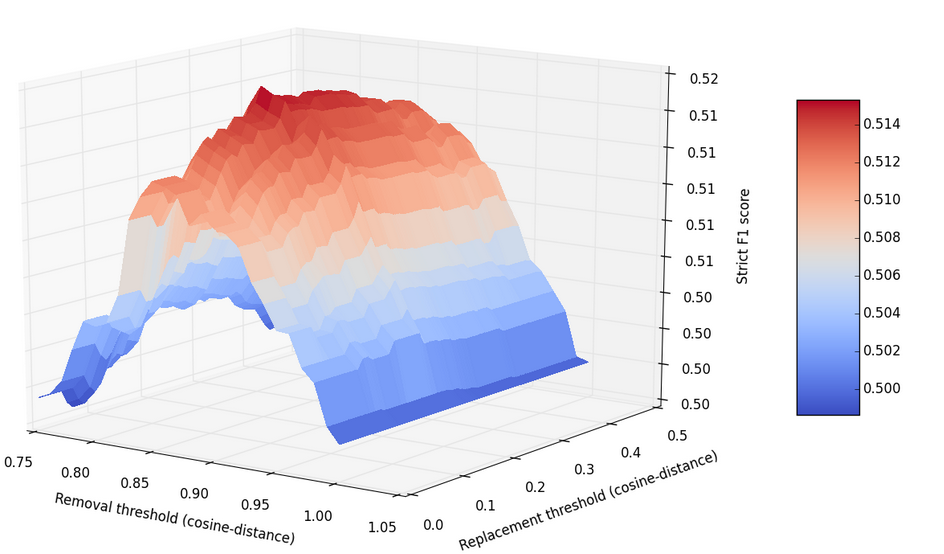
\includegraphics[width=0.5\textwidth]{gridsearch.png}
\caption{Strict $F_1$ score of different thresholds on the training set. The optimal values are $0.85$ and $0.2$.}
\label{fig:gridsearch}
\end{figure}

\section{Results}
In table \ref{tbl:results} you can see our results in terms of strict and lazy $F_1$ score on the training and dev data sets. Our system approaches the performance of tagme on the train data set and surpasses it on the dev data set.



\begin{table}[H]
\centering
\begin{tabular}{|l|r|r|r|r|}
\hline
 &  \multicolumn{2}{c|}{\textbf{Train data set}} & \multicolumn{2}{c|}{\textbf{Dev data set}} \\
\hline
 & Strict $F_1$ & Lazy $F_1$ & Strict $F_1$ & Lazy $F_1$ \\
\hline
\textbf{Naive} & 0.385 & 0.429 & 0.431 & 0.495 \\
\textbf{Tagme} & 0.545 & 0.615 & 0.543 & 0.610 \\
\textbf{LDA} & 0.516 & 0.575 & 0.543 & 0.619 \\
\hline
\end{tabular}
\caption{Results of the naive annotator, the tagme annotator and the LDA-based annotator in terms of strict and lazy $F_1$ score.}
\label{tbl:results}
\end{table}


\section{Conclusion \& Future Work}
Annotating simply with the highest prior annotation turned out to give the best results. A reason for this could be the simplicity of an average query, i.e. people usually look for the most common things. Moreover, the evaluation depends very much on having the correct entity set. As not every entity used by the human annotator is included in the entity set of the crosswiki file, it is impossible to get 100\% correct annotations. We measured that our theoretical upper bound is 72.3\%. In addition, LDA is able to help removing false positives and in some cases replace false positives with true positives.



\end{document}